\documentclass[conference]{IEEEtran}
\IEEEoverridecommandlockouts
% The preceding line is only needed to identify funding in the first footnote. If that is unneeded, please comment it out.
\usepackage[backend=biber]{biblatex}
\addbibresource{references.bib}
\usepackage{amsmath,amssymb,amsfonts}
\usepackage{algorithmic}
\usepackage{graphicx}
\usepackage{textcomp}
\usepackage{xcolor}
\usepackage{hyperref}
\def\BibTeX{{\rm B\kern-.05em{\sc i\kern-.025em b}\kern-.08em
    T\kern-.1667em\lower.7ex\hbox{E}\kern-.125emX}}
\begin{document}

\title{Audio Super-Resolution\\
}

\author{
\IEEEauthorblockN{Şut George-Mihai}
\IEEEauthorblockA{\textit{3rd-year undergraduate, Computer Science} \\
\textit{Babeş-Bolyai University}\\
georgesut@yahoo.com}
}

\maketitle

\begin{abstract}
Audio super-resolution refers to the task of increasing the sampling rate of an audio signal by training a neural net to produce outputs whose sampling rate is higher by a specific factor (x2, x4, x6 etc.).
\end{abstract}

\section{Introduction}
	In this paper, the goal is to investigate on whether a neural net can be trained with low-resolution audio data given as an input to produce super-resolution audio (i.e a reconstructed high-resolution audio signal). The point of the model is to predict the samples which are missing from the audio signal, which in this case will consist of short, downsampled pieces of music collected from a publicly available API. The project has been inspired by image super-resolution and especially by time-series super-resolution, which in essence operates with the same methods for generating the training dataset by downsampling high-resolution data and making use of a generative model to reconstruct a signal. (\textcite{kuleshov2017audio}, \textcite{hetherly2017audio})

	The process of audio super-resolution using neural nets (also called bandwidth extension) is explained in \textcite{kuleshov2017audio} which states that the goal is to reconstruct a low-resolution signal with a sample rate $ R_{1} $ into a high-resolution signal with a greater sample rate $ R_{2} $. The paper clarifies the concept by giving a simple example of a 4 KHz signal being upsampled through audio super-resolution to a 16 KHz signal by a factor of 4. The audio signal is encoded into a spectrogram which displays the frequencies contained in the signal and the sound intensity in decibels. 

	For the model, a bottleneck-type architecture has been used, similar to the U-Net architecture, containing residual connections between pairs of layer $ b $ and layer $ B - b + 1 $, where $ B $ is the number of layers in the network. The first part of the network is responsible for downsampling data, whereas the second part upsamples it. The experiment conducted on the MagnaTagATune dataset in \textcite{kuleshov2017audio} shows that applying this architecture on music leads to poor results which could be improved with a larger and more computationally demanding model, so the model is mostly suitable only for vocal recordings, meaning that it can be useful in voice-over-IP applications.

	The second article (\textcite{hetherly2017audio}) mentions that the presented implementation has only been trained on 10 epochs, hence the mediocre outputs, compared to the 400-epoch model described by \textcite{kuleshov2017audio}

	
\begin{figure}[htbp]
		\centerline{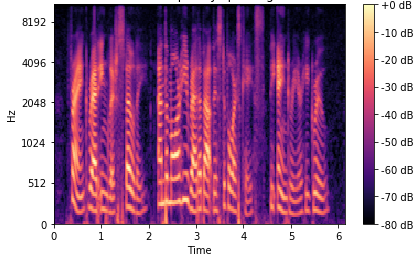
\includegraphics[width=9.5cm,height=5.5cm]{spectrogram.png}}
\caption{Example of a spectrogram where time is shown on the $ x $ axis, the frequencies out of which the signal is composed are shown on the $ y $ axis and their corresponding magnitudes in decibels are displayed in the colorbar on the right.}
\label{fig}
\end{figure}



		
\printbibliography
\vspace{12pt}

\end{document}

